\documentclass{beamer}
\usepackage{graphicx}
\usepackage[english]{babel}
\usepackage{multicol}
\usepackage{animate}
\usepackage{xcolor}

\usepackage{booktabs}   %% For formal tables:
%% http://ctan.org/pkg/booktabs
\usepackage{subcaption} %% For complex figures with subfigures/subcaptions
%% http://ctan.org/pkg/subcaption
\usepackage[export]{adjustbox}

\usepackage[T1]{fontenc} % fix missing font cmtt
\usepackage{amsmath}
\let\Bbbk\relax
\usepackage{amssymb} % Vdash
\usepackage{graphicx} % rotatebox
\usepackage{stmaryrd} % llparenthesis
\usepackage{anyfontsize} % workaround for font size difference warning
\usepackage{todonotes}
\usepackage{listings}
\usepackage{tikz}
\usetikzlibrary{calc,fit,tikzmark,plotmarks,arrows.meta,positioning,overlay-beamer-styles}

\usepackage{cancel} % slash over symbol
\usepackage{hyperref}
\renewcommand\UrlFont{\color{blue}\rmfamily}
\def\figureautorefname{Fig.}
\def\lemmaautorefname{Lemma}
\def\sectionautorefname{Sec.}
\let\subsectionautorefname\sectionautorefname
\let\subsubsectionautorefname\sectionautorefname
\newcommand{\rulesref}[1]{Rules (\ref{#1})}
\newcommand{\ruleref}[1]{Rule (\ref{#1})}

\usepackage{xcolor}
\definecolor{hazelgreen}{RGB}{7,63,36}
\definecolor{hazellightgreen}{RGB}{103,138,97}
\definecolor{hazelyellow}{RGB}{245,222,179}
\definecolor{hazellightyellow}{RGB}{254,254,234}

\newcommand{\highlight}[1]{\colorbox{yellow}{$\displaystyle #1$}}

%% Jana Dunfield macros
\def\OPTIONConf{1}
\usepackage{jdunfield}
\usepackage{rulelinks}

\usepackage{listings}%
\lstloadlanguages{ML}
\lstset{tabsize=2, 
	basicstyle=\fontsize{7.5pt}{1em}\ttfamily, 
	% keywordstyle=\sffamily,
	commentstyle=\itshape\ttfamily\color{gray}, 
	stringstyle=\ttfamily\color{purple},
	mathescape=true,escapechar=\#,
	numbers=left, numberstyle=\scriptsize\color{gray}\ttfamily, language=ML, showspaces=false,showstringspaces=false,xleftmargin=15pt, 
	morekeywords={string, float, int, bool, match},
	classoffset=0,belowskip=\smallskipamount, aboveskip=\smallskipamount,
	moredelim=**[is][\color{red}]{SSTR}{ESTR}
}
\newcommand{\li}[1]{\lstinline[basicstyle=\ttfamily\fontsize{9pt}{1em}\selectfont]{#1}}
\newcommand{\lismall}[1]{\lstinline[basicstyle=\ttfamily\fontsize{9pt}{1em}\selectfont]{#1}}

% !TEX root = proposal.tex
\usepackage{centernot}
% reverse Vdash
\newcommand{\dashV}{\mathbin{\rotatebox[origin=c]{180}{$\Vdash$}}}

% Violet hotdogs; highlight color helps distinguish them
\newcommand{\llparenthesiscolor}{\textcolor{violet}{\llparenthesis}}
\newcommand{\rrparenthesiscolor}{\textcolor{violet}{\rrparenthesis}}

% HTyp and HExp
\newcommand{\hcomplete}[1]{#1~\mathsf{complete}}

% HTyp
\newcommand{\htau}{\dot{\tau}}
\newcommand{\tarr}[2]{\inparens{#1 \rightarrow #2}}
\newcommand{\tarrnp}[2]{#1 \rightarrow #2}
\newcommand{\trul}[2]{\inparens{#1 \Rightarrow #2}}
\newcommand{\trulnp}[2]{#1 \Rightarrow #2}
\newcommand{\tnum}{\mathtt{num}}
\newcommand{\tehole}{\llparenthesiscolor\rrparenthesiscolor}
\newcommand{\tsum}[2]{\inparens{#1 + #2}}
\newcommand{\tprod}[2]{\inparens{#1 \times #2}}
\newcommand{\tunit}{\mathtt{1}}
\newcommand{\tvoid}{\mathtt{0}}

\newcommand{\tlabeledsum}[1]{+\mathopen{}\left\{#1\right\}}

\newcommand{\tcompat}[2]{#1 \sim #2}
\newcommand{\tincompat}[2]{#1 \nsim #2}


% HTag
\newcommand{\tagC}{\underline{\mathbf{C}}}
\newcommand{\tagset}{\mathcal{C}}
\newcommand{\tagehole}[1]{\llparenthesiscolor\rrparenthesiscolor^{#1}}
\newcommand{\taghole}[2]{\llparenthesiscolor#1\rrparenthesiscolor^{#2}}

\newcommand{\tagmaymatch}[2]{#1 \mathbin{?} #2}

% HExp
\newcommand{\hexp}{\dot{e}}
\newcommand{\hlam}[3]{\lambda #1:#2.#3}
\newcommand{\hap}[2]{#1(#2)}
\newcommand{\hapP}[2]{(#1)~(#2)} % Extra paren around function term
\newcommand{\hnum}[1]{\underline{#1}}
\newcommand{\hadd}[2]{\inparens{#1 + #2}}
\newcommand{\hpair}[2]{(#1 , #2)}
\newcommand{\htriv}{()}
\newcommand{\hehole}[1]{\llparenthesiscolor\rrparenthesiscolor^{#1}}
\newcommand{\hhole}[2]{\llparenthesiscolor#1\rrparenthesiscolor^{#2}}
\newcommand{\heholep}[1]{\llparenthesiscolor\rrparenthesiscolor^{#1}}
\newcommand{\hholep}[3]{\llparenthesiscolor#1\rrparenthesiscolor^{#2}_{#3}}
\newcommand{\hindet}[1]{\lceil#1\rceil}
\newcommand{\hinj}[3]{\mathtt{inj}_{#1}^{#2}({#3})}
\newcommand{\hinl}[2]{\mathtt{inl}_{#1}({#2})}
\newcommand{\hinr}[2]{\mathtt{inr}_{#1}({#2})}
\newcommand{\hinjp}[2]{\mathtt{inj}_{#1}(#2)}
\newcommand{\hinlp}[1]{\mathtt{inl}(#1)}
\newcommand{\hinrp}[1]{\mathtt{inr}(#1)}
\newcommand{\hfst}[1]{\mathtt{fst}(#1)}
\newcommand{\hsnd}[1]{\mathtt{snd}(#1)}
\newcommand{\hmatch}[2]{\mathtt{match}(#1) \{#2\}}
\newcommand{\hcase}[5]{\mathtt{case}({#1},{#2}.{#3},{#4}.{#5})}
\newcommand{\hrules}[2]{#1 \mid #2}
\newcommand{\hrulesP}[2]{\inparens{#1 \mid #2}}
\newcommand{\hrul}[2]{#1 \Rightarrow #2}
\newcommand{\hrulP}[2]{\inparens{#1 \Rightarrow #2}}

\newcommand{\refutable}[1]{#1 ~\mathtt{refutable}_?}
\newcommand{\frefutable}[1]{\textit{refutable}_?\inparens{#1}}
\newcommand{\possible}[1]{#1 ~\mathtt{possible}}
\newcommand{\fpossible}[1]{\textit{possible}\inparens{#1}}
\newcommand{\inValues}[3]{#1 \in \mathtt{values}[#2]\inparens{#3}}

\newcommand{\hGamma}{\dot{\Gamma}}
\newcommand{\domof}[1]{\text{dom}(#1)}
\newcommand{\hsyn}[3]{#1 \vdash #2 \Rightarrow #3}
\newcommand{\hana}[3]{#1 \vdash #2 \Leftarrow #3}
\newcommand{\hexptyp}[4]{#1 \mathbin{;} #2 \vdash #3 : #4}
\newcommand{\hpattyp}[4]{#4 \vdash #1 : #2 \dashV #3}
\newcommand{\hsubstyp}[4]{#1 \mathbin{;} #2 \vdash #3 : #4}
\newcommand{\hpatmatch}[3]{#1 \vartriangleright #2 \dashV #3}
\newcommand{\hnotnotmatch}[2]{#1 \mathbin{\cancel{\bot}} #2}
\newcommand{\hnotmatch}[2]{#1 \mathbin{\bot} #2}
\newcommand{\hmaymatch}[2]{#1 \mathbin{?} #2}
\newcommand{\htrans}[2]{#1 \mapsto #2}
\newcommand{\hlongtrans}[2]{#1 \newline \mapsto #2}

\newcommand{\isVal}[1]{#1 ~\mathtt{val}}
\newcommand{\isErr}[1]{#1 ~\mathtt{err}}
\newcommand{\isIndet}[1]{#1 ~\mathtt{indet}}
\newcommand{\isFinal}[1]{#1 ~\mathtt{final}}
\newcommand{\notIntro}[1]{#1 ~\mathtt{notintro}}
\newcommand{\fnotIntro}[1]{\textit{notintro}\inparens{#1}}

\newcommand{\setof}[1]{\{#1\}}

% ZTyp and ZExp
\newcommand{\zlsel}[1]{{\bowtie}{#1}}
\newcommand{\zrsel}[1]{{#1}{\bowtie}}
\newcommand{\zwsel}[1]{
	\setlength{\fboxsep}{0pt}
	\colorbox{green!10!white!100}{
		\ensuremath{{{\textcolor{Green}{{\hspace{-2px}\triangleright}}}}{#1}{\textcolor{Green}{\triangleleft{\vphantom{\tehole}}}}}}
}

\newcommand{\removeSel}[1]{#1^{\diamond}}

% ZTyp
\newcommand{\ztau}{\hat{\tau}}

% ZExp
\newcommand{\zexp}{\hat{e}}

% rules with pointer

\newcommand{\zrulsP}[3]{\inparens{#1 \mid #2 \mid #3}}
\newcommand{\zruls}[3]{#1 \mid #2 \mid #3}
\newcommand{\zrules}{\hat{rs}}
\newcommand{\rmpointer}[1]{\inparens{#1}^\diamond}

% Constraint
\newcommand{\hxi}{\dot{\xi}}
\newcommand{\ctyp}[2]{#1 : #2}
\newcommand{\cdual}[1]{\overline{#1}}
\newcommand{\ctruify}[1]{\dot{\top}\inparens{#1}}
\newcommand{\cfalsify}[1]{\dot{\bot}\inparens{#1}}
\newcommand{\ctruth}{\top}
\newcommand{\cfalsity}{\bot}
\newcommand{\cnum}[1]{\underline{#1}}
\newcommand{\cnotnum}[1]{\underline{\cancel{#1}}}
\newcommand{\cunit}{()}
\newcommand{\cunknown}{\mathtt{?}}
\newcommand{\cor}[2]{#1 \vee #2}
\newcommand{\cand}[2]{#1 \wedge #2}
\newcommand{\cinj}[3]{\mathtt{inj}_{#1}^{#2}(#3)}
\newcommand{\notC}{\cancel{C}}
\newcommand{\nottagC}{\cancel{\tagC}}
\newcommand{\cinl}[1]{\mathtt{inl}(#1)}
\newcommand{\cinr}[1]{\mathtt{inr}(#1)}
\newcommand{\cpair}[2]{(#1 , #2)}
\newcommand{\csatisfy}[2]{#1 \models #2}
\newcommand{\cnotsatisfy}[2]{#1 \centernot{\models} #2}
\newcommand{\cmaysatisfy}[2]{#1 \models_{?} #2}
\newcommand{\cnotmaysatisfy}[2]{#1 \centernot{\models}_{?} #2}
\newcommand{\csatisfyormay}[2]{#1 \models_{?}^{\dag} #2}
\newcommand{\cnotsatisfyormay}[2]{#1 \centernot{\models}_{?}^{\dag} #2}
%temporary change, need to get it back to make appendix right
%\newcommand{\csatisfy}[2]{#1 \dot{\models} #2}
%\newcommand{\cnotsatisfy}[2]{#1 \centernot{\dot{\models}} #2}
%\newcommand{\cmaysatisfy}[2]{#1 \dot{\models}_{?} #2}
%\newcommand{\cnotmaysatisfy}[2]{#1 \centernot{\dot{\models}}_{?} #2}
%\newcommand{\csatisfyormay}[2]{#1 \dot{\models}_{?}^{\dag} #2}
%\newcommand{\cnotsatisfyormay}[2]{#1 \centernot{\dot{\models}}_{?}^{\dag} #2}
\newcommand{\ccsatisfy}[2]{#1 \models #2}
\newcommand{\ccnotsatisfy}[2]{#1 \centernot{\models} #2}
\newcommand{\cincon}[1]{#1 ~\mathtt{incon}}
\newcommand{\cmayincon}[1]{#1 ~\cancel{\mathtt{not~incon}}}

\newcommand{\fsatisfy}[2]{\textit{satisfy}\inparens{#1, #2}}
% !TeX root = thesis.tex
%% Statics

% typing of internal expressions
\newrulecommand{TVar}{TVar}
\newrulecommand{TNum}{TNum}
\newrulecommand{TLam}{TLam}
\newrulecommand{TAp}{TAp}
\newrulecommand{TPair}{TPair}
\newrulecommand{TFst}{TFst}
\newrulecommand{TSnd}{TSnd}
\newrulecommand{TInl}{TInl}
\newrulecommand{TInr}{TInr}
\newrulecommand{TMatchZPre}{TMatchZPre}
\newrulecommand{TMatchNZPre}{TMatchNZPre}
\newrulecommand{TEHole}{TEHole}
\newrulecommand{THole}{THole}

% typing of rule and rules
\newrulecommand{TRule}{TRule}
\newrulecommand{TOneRules}{TOneRules}
\newrulecommand{TRules}{TRules}

% typing of pattern
\newrulecommand{PTVar}{PTVar}
\newrulecommand{PTNum}{PTNum}
\newrulecommand{PTWild}{PTWild}
\newrulecommand{PTPair}{PTPair}
\newrulecommand{PTInl}{PTInl}
\newrulecommand{PTInr}{PTInr}
\newrulecommand{PTEHole}{PTEHole}
\newrulecommand{PTHole}{PTHole}

%% Dynamics

% typing of substitution
\newrulecommand{STEmpty}{STEmpty}
\newrulecommand{STExtend}{STExtend}

% syntactically not value
\newrulecommand{NVEHole}{NVEHole}
\newrulecommand{NVHole}{NVHole}
\newrulecommand{NVAp}{NVAp}
\newrulecommand{NVMatch}{NVMatch}
\newrulecommand{NVFst}{NVFst}
\newrulecommand{NVSnd}{NVSnd}

% refutable pattern
\newrulecommand{RNum}{RNum}
\newrulecommand{REHole}{REHole}
\newrulecommand{RHole}{RHole}
\newrulecommand{RInl}{RInl}
\newrulecommand{RInr}{RInr}
\newrulecommand{RPairL}{RPairL}
\newrulecommand{RPairR}{RPairR}

% refutable constraint
\newrulecommand{RXNum}{RXNum}
\newrulecommand{RXNotNum}{RXNotNum}
\newrulecommand{RXUnknown}{RXUnknown}
\newrulecommand{RXFalsity}{RXFalsity}
\newrulecommand{RXInl}{RXInl}
\newrulecommand{RXInr}{RXInr}
\newrulecommand{RXPairL}{RXPairL}
\newrulecommand{RXPairR}{RXPairR}

% possible constraint
\newrulecommand{PTruth}{PTruth}
\newrulecommand{PUnknown}{PUnknown}
\newrulecommand{PNum}{PNum}
\newrulecommand{PNotNum}{PNotNum}
\newrulecommand{PInl}{PInl}
\newrulecommand{PInr}{PInr}
\newrulecommand{PPair}{PPair}
\newrulecommand{POrL}{POrL}
\newrulecommand{POrR}{POrR}

% match
\newrulecommand{MVar}{MVar}
\newrulecommand{MNum}{MNum}
\newrulecommand{MWild}{MWild}
\newrulecommand{MPair}{MPair}
\newrulecommand{MNotIntroPair}{MNotIntroPair}
\newrulecommand{MInl}{MInl}
\newrulecommand{MInr}{MInr}

% may match
\newrulecommand{MMEHole}{MMEHole}
\newrulecommand{MMHole}{MMHole}
\newrulecommand{MMNotIntro}{MMNotIntro}
\newrulecommand{MMPairL}{MMPairL}
\newrulecommand{MMPairR}{MMPairR}
\newrulecommand{MMPair}{MMPair}
\newrulecommand{MMInl}{MMInl}
\newrulecommand{MMInr}{MMInr}

% not match
\newrulecommand{NMNum}{NMNum}
\newrulecommand{NMPairL}{NMPairL}
\newrulecommand{NMPairR}{NMPairR}
\newrulecommand{NMConfL}{NMConfL}
\newrulecommand{NMConfR}{NMConfR}
\newrulecommand{NMInl}{NMInl}
\newrulecommand{NMInr}{NMInr}

% value
\newrulecommand{VNum}{VNum}
\newrulecommand{VLam}{VLam}
\newrulecommand{VPair}{VPair}
\newrulecommand{VInl}{VInl}
\newrulecommand{VInr}{VInr}

% indeterminate
\newrulecommand{IEHole}{IEHole}
\newrulecommand{IHole}{IHole}
\newrulecommand{IAp}{IAp}
\newrulecommand{IPairL}{IPairL}
\newrulecommand{IPairR}{IPairR}
\newrulecommand{IPair}{IPair}
\newrulecommand{IFst}{IFst}
\newrulecommand{ISnd}{ISnd}
\newrulecommand{IInl}{IInl}
\newrulecommand{IInr}{IInr}
\newrulecommand{IMatch}{IMatch}

% final
\newrulecommand{FVal}{FVal}
\newrulecommand{FIndet}{FIndet}

% step
\newrulecommand{ITHole}{ITHole}
\newrulecommand{ITApFun}{ITApFun}
\newrulecommand{ITApArg}{ITApArg}
\newrulecommand{ITAp}{ITAp}
\newrulecommand{ITPairL}{ITPairL}
\newrulecommand{ITPairR}{ITPairR}
\newrulecommand{ITFst}{ITFst}
\newrulecommand{ITSnd}{ITSnd}
\newrulecommand{ITFstPair}{ITFstPair}
\newrulecommand{ITSndPair}{ITSndPair}
\newrulecommand{ITInl}{ITInl}
\newrulecommand{ITInr}{ITInr}
\newrulecommand{ITExpMatch}{ITExpMatch}
\newrulecommand{ITSuccMatch}{ITSuccMatch}
\newrulecommand{ITFailMatch}{ITFailMatch}

% typing of constraints
\newrulecommand{CTTruth}{CTTruth}
\newrulecommand{CTFalsity}{CTFalsity}
\newrulecommand{CTUnknown}{CTUnknown}
\newrulecommand{CTNum}{CTNum}
\newrulecommand{CTNotNum}{CTNotNum}
\newrulecommand{CTAnd}{CTAnd}
\newrulecommand{CTOr}{CTOr}
\newrulecommand{CTInl}{CTInl}
\newrulecommand{CTInr}{CTInr}
\newrulecommand{CTPair}{CTPair}

% satisfaction judgment
\newrulecommand{CSTruth}{CSTruth}
\newrulecommand{CSNum}{CSNum}
\newrulecommand{CSNotNum}{CSNotNum}
\newrulecommand{CSAnd}{CSAnd}
\newrulecommandONE{CSOrL}{CSOrL}
\newrulecommandONE{CSOrR}{CSOrR}
\newrulecommand{CSInl}{CSInl}
\newrulecommand{CSInr}{CSInr}
\newrulecommand{CSPair}{CSPair}
\newrulecommand{CSNotIntroPair}{CSNotIntroPair}

% maybe satisfaction judgment
\newrulecommand{CMSUnknown}{CMSUnknown}
\newrulecommand{CMSNotIntro}{CMSNotIntro}
\newrulecommand{CMSAndL}{CMSAndL}
\newrulecommand{CMSAndR}{CMSAndR}
\newrulecommand{CMSAnd}{CMSAnd}
\newrulecommand{CMSOrL}{CMSOrL}
\newrulecommand{CMSOrR}{CMSOrR}
\newrulecommand{CMSInl}{CMSInl}
\newrulecommand{CMSInr}{CMSInr}
\newrulecommand{CMSPairL}{CMSPairL}
\newrulecommand{CMSPairR}{CMSPairR}
\newrulecommand{CMSPair}{CMSPair}

% must or maybe satisfaction judgment
\newrulecommand{CSMSMay}{CSMSMay}
\newrulecommand{CSMSSat}{CSMSSat}

% incon
\newrulecommand{CINCTruth}{CINCTruth}
\newrulecommand{CINCFalsity}{CINCFalsity}
\newrulecommand{CINCNum}{CINCNum}
\newrulecommand{CINCNotNum}{CINCNotNum}
\newrulecommand{CINCAnd}{CINCAnd}
\newrulecommand{CINCOr}{CINCOr}
\newrulecommand{CINCInj}{CINCInj}
\newrulecommand{CINCInl}{CINCInl}
\newrulecommand{CINCInr}{CINCInr}
\newrulecommand{CINCPairL}{CINCPairL}
\newrulecommand{CINCPairR}{CINCPairR}

%% labeled sum dynamics
\newrulecommand{ITInj}{ITInj}
\newrulecommand{VInj}{VInj}
\newrulecommand{IEInj}{IEInj}
\newrulecommand{IEInjHole}{IEInjHole}
\newrulecommand{MInj}{MInj}
\newrulecommand{NMInj}{NMInj}
\newrulecommand{NMInjTag}{NMInjTag}
\newrulecommand{NMInjArg}{NMInjArg}
\newrulecommand{MMInjTag}{MMInjTag}
\newrulecommand{MMInjArg}{MMInjArg}
\newrulecommand{TMMSym}{TMMSym}
\newrulecommand{TMMHole}{TMMHole}
\newrulecommand{TMMEHole}{TMMEHole}
\newrulecommand{TNMTag}{TNMTag}
\newrulecommand{RInjSing}{RInjSing}
\newrulecommand{RInjMult}{RInjMult}

% labeled sum statics
\newrulecommand{TInj}{TInj}
\newrulecommand{PTInj}{PTInj}
\newrulecommand{CTInj}{CTInj}
\newrulecommand{RXInj}{RXInj}
\newrulecommand{PInj}{PInj}
\newrulecommand{CSInj}{CSInj}
\newrulecommand{CMSInjTag}{CMSInjTag}
\newrulecommand{CMSInjArg}{CMSInjArg}

% labeled sum incon
\newrulecommand{CINCInjTag}{CINCInjTag}
\newrulecommand{CINCInjArg}{CINCInjArg}

% Curry-Howard Correspondence
\newrulecommand{AndIntro}{AndIntro}
\newrulecommand{AndElimL}{AndElimL}
\newrulecommand{AndElimR}{AndElimR}
\newrulecommand{TAPair}{TAPair}
\newrulecommand{TAFst}{TAFst}
\newrulecommand{TASnd}{TASnd}

\newrulecommand{UniversalIntro}{UniversalIntro}
\newrulecommand{UniversalElim}{UniversalElim}
\newrulecommand{TALam}{TALam}
\newrulecommand{TAAp}{TAAp}

% Agda examples
\newrulecommand{Zero}{Zero}
\newrulecommand{Suc}{Suc}
\newrulecommand{ZLessThanS}{Z<S}
\newrulecommand{SLessThanS}{S<S}

% BadRules
\newrulecommand{BadTRule}{BadTRule}
\newrulecommand{GoodTRule}{GoodTRule}


\mode<presentation>
{ 
	\usetheme{AnnArbor}
    \usecolortheme{default}
    \usefonttheme{structurebold}
}

%gets rid of bottom navigation bars
\setbeamertemplate{footline}[frame number]{}

%gets rid of bottom navigation symbols
\setbeamertemplate{navigation symbols}{}

%gets rid of footer
%will override 'frame number' instruction above
%comment out to revert to previous/default definitions
\setbeamertemplate{footline}{}

\title[Computer Science Honors Thesis]{Pattern Matching with Typed Holes}
\author{Yongwei Yuan, \underline{Scott Guest}, Eric Griffis, Hannah Potter, David Moon, Cyrus Omar}
\institute{University of Michigan}
\date{8 April 2022}

\begin{document}
\begin{frame}
\titlepage
\end{frame}

%\begin{frame}
%	\frametitle{Sum Types}
%	\begin{itemize}
%		\item Sum types give an "or" of types - similar to enums, but each tag can also hold data
%		\medskip
%		\begin{itemize}
%			\item Type: \li{sum \{Good([Int]) + Error(String)\}}
%			\medskip
%			\item Values: \li{Good([])}, \li{Good([1, 2, 3, 4])}, \li{Error("bad list")}, ...
%		\end{itemize}
%		\medskip
%		\item Linked lists are sum types with special syntax
%		\medskip
%		\begin{itemize}
%			\item \li{IntList} defined as \li{sum \{Node(Int, IntList) + Empty\}}
%			\medskip
%			\item \li{Node(hd, tl)} written as \li{hd::tl}
%			\medskip
%			\item \li{Empty} written as \li{[]}
%			\medskip
%			\item \li{[1, 2, 3, 4]} desguars to \li{1::2::3::4::[]}
%		\end{itemize}
%	\end{itemize}
%\end{frame}

%\begin{frame}
%\frametitle{Pattern Matching}
%\begin{itemize}
%\item A pattern specifies a certain "shape" for values of a sum type, with variables akin to wildcards
%\medskip
%\begin{itemize}
%	\item \li{[1, 2, 3, 4]} matches the pattern \li{hd::tl}
%	\medskip
%	\item \li{[1]} does not match the pattern \li{x::y::tl}
%	\medskip
%	\item \li{Good([1, 2, 3, 4])} matches the pattern \li{Good(x::y::tl)}
%	\medskip
%	\item \li{Error("bad list")} does not match the pattern \li{Good(xs)}
%\end{itemize}
%\medskip
%\item Match expressions compare a scrutinee against a sequence of patterns, selecting the branch of the first pattern that matches
%\medskip
%\item Exhaustiveness - every expression matches at least one pattern
%\medskip
%\item Irredundancy - every pattern is matched by at least one expression
%\end{itemize}
%\end{frame}

\begin{frame}
\frametitle{Pattern Matching}
\begin{itemize}
\item A pattern specifies a particular "shape" than an expression can take, with variables treated as wildcards
\medskip
\item Match expressions compares a \emph{scrutinee} against a sequence of \emph{rules}, where each rule consists of a pattern and a branch expression.
\medskip
\begin{itemize}
\item Proceeds top down, evaluating to the branch expression of the first matched pattern
\end{itemize}
\medskip
\item Exhaustiveness - every expression matches at least one pattern
\medskip
\item Irredundancy - every pattern is matched by at least one expression
\end{itemize}
\end{frame}
\begin{frame}
	\frametitle{Typed Holes}
	\begin{itemize}
	\item Problem: Editor services struggle to deal with unfinished programs because they are formally meaningless
	\medskip
	\item Hazel represents unfinished programs as terms with holes 
	\medskip
		\begin{itemize}
			\item Empty holes $\hehole{u}$ indicate missing syntactic pieces 
			\medskip
			\item Non-empty holes $\hhole{e}{u}$ surround semantic inconsistencies 
		\end{itemize}
	\medskip
	\item Maximal Liveness - Every editor state has static and dynamic meaning
	\medskip
	\item Give terms as much meaning as possible, being conservative with respect to all hole-fillings
	\end{itemize}
%	\begin{figure}
%		\centering
%		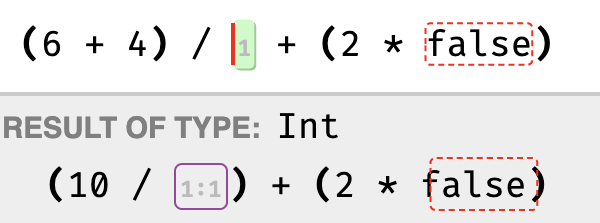
\includegraphics[scale=0.47,valign=t]{imgs/arith-initial.png}%
%%		\hfill
%%		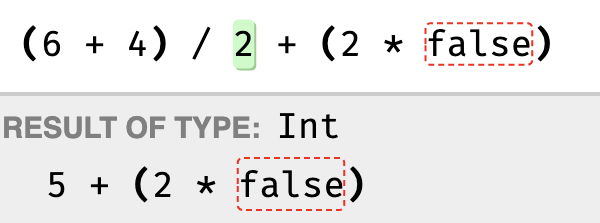
\includegraphics[scale=0.47,valign=t]{imgs/arith-partial.png}%
%		\caption{Live Evaluation with Expression Holes}
%	\end{figure}
\end{frame}

\begin{frame}
\frametitle{Pattern Matching with Holes}
\begin{itemize}
\item Use empty pattern holes $\heholep{w}$ and non-empty pattern holes $\hholep{p}{w}{\tau}$ to represent intermediate pattern edit states\\
\medskip
\item $\hpatmatch{e}{p}{\theta}$ - in all hole-fillings, $e$ matches $p$, emitting bindings $\theta$\\

\begin{itemize}
\item $1::\hehole{u}::[~]$ must match $hd :: tl$, binding $hd$ to $1$ and $tl$ to $\hehole{u}::[~]$
\end{itemize}
\medskip
\item $\hnotmatch{e}{p}$ - in all hole-fillings, $e$ does not match $p$\\

\begin{itemize}
\item $1::[~]$ must not match $x::\heholep{w}::tl$
\end{itemize}
\medskip
\item $\hmaymatch{e}{p}$ - depending on the hole-filling, $e$ may or may not match $p$\\

\begin{itemize}
\item $1::[~]$ indeterminately matches $\heholep{w}::[~]$\\
\end{itemize}
\end{itemize}
\end{frame}

\begin{frame}
\frametitle{Pattern Matching with Holes}
\begin{figure}
	\centering
	% Capture tallest image in box 2
	\setbox2=\hbox{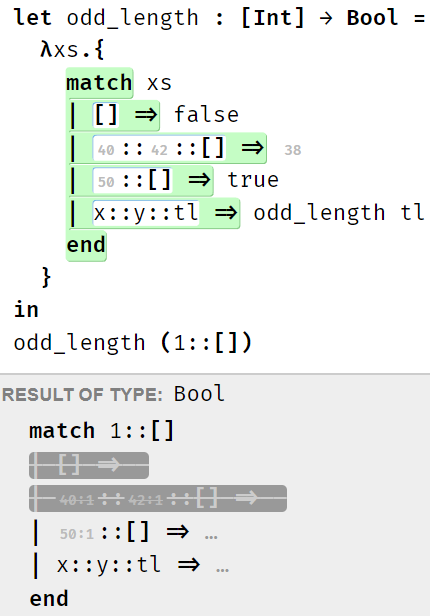
\includegraphics[scale=0.5]{imgs/pat_match_pat_holes.png}}%
	\subcaptionbox{Expression Holes\label{fig:exp-hole}}{
		\raisebox{\dimexpr\ht2-\height}{
			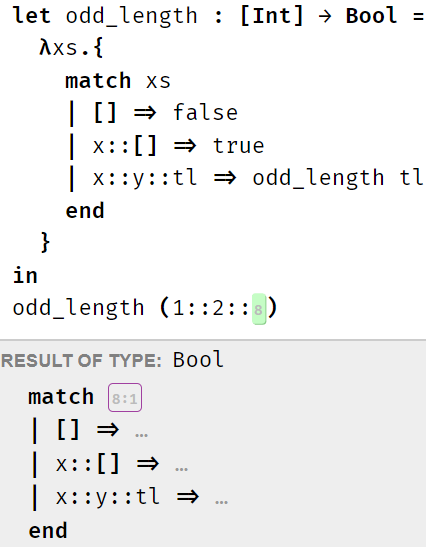
\includegraphics[scale=0.5,valign=t]{imgs/pat_match_exp_holes.png}
			\vphantom{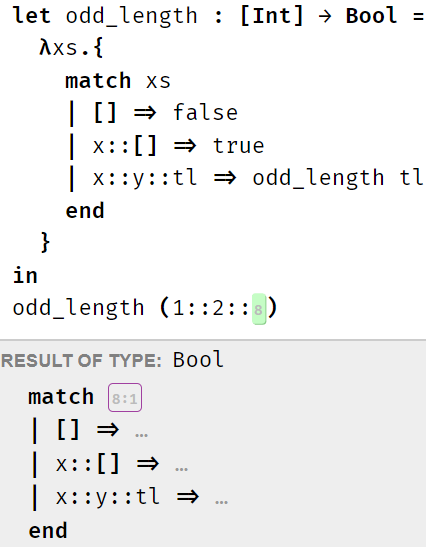
\includegraphics[scale=0.47,valign=t]{imgs/pat_match_exp_holes.png}}
		}
	}
	\hfil
	\subcaptionbox{Pattern Holes\label{fig:pat-hole}}{
		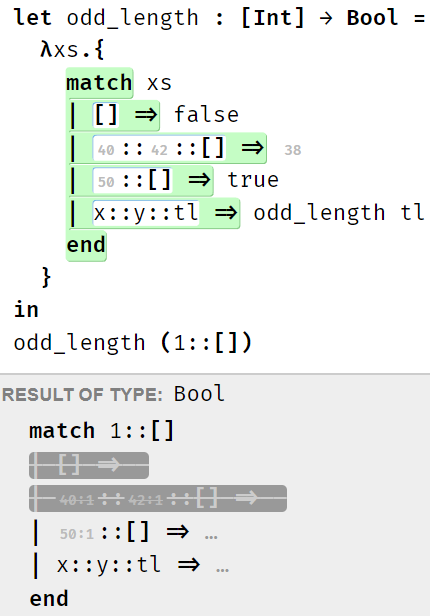
\includegraphics[scale=0.5,valign=t]{imgs/pat_match_pat_holes.png}
	}
\end{figure}
\end{frame}

\begin{frame}
\frametitle{The Peanut Calculus}
\begin{itemize}
\item Lambda calculus with numbers, binary products, and binary sums
\item Represent intermediate match states with a "zippered" list of rules
\end{itemize}
% !TeX root = presentation.tex

\begin{figure}[ht]
    \centering
    \begin{minipage}{.5\linewidth}
  $\arraycolsep=4pt\begin{array}{lll}
    e & ::= &
      x ~\vert~
      \hnum{n} \\
      & ~\vert~ &
      \hlam{x}{\tau}{e} ~\vert~
      \hap{e_1}{e_2} \\
      & ~\vert~ &
      \hpair{e_1}{e_2} ~\vert~
      \hfst{e} ~\vert~ \hsnd{e} \\
      & ~\vert~ &
      \hinl{\tau}{e} ~\vert~
      \hinr{\tau}{e} \\
      & ~\vert~ &
      \hmatch{e}{\hat{rs}} \\
      & ~\vert~ &
      \hehole{u} ~\vert~
      \hhole{e}{u} \\
    \end{array}$
    \end{minipage}%
    \begin{minipage}{.5\linewidth}
  $\arraycolsep=4pt\begin{array}{lll}
    \tau & ::= &
      \tnum ~\vert~
      \tarr{\tau_1}{\tau_2}\\
      & ~\vert~ &
      \tprod{\tau_1}{\tau_2} ~\vert~
      \tsum{\tau_1}{\tau_2} \\
    \hat{rs} & ::= &
      \zrulsP{rs}{r}{rs} \\
    rs & ::= &
      \cdot ~\vert~ \hrulesP{r}{rs'} \\
    r & ::= &
      \hrul{p}{e} \\
    p & ::= &
      x ~\vert~
      \_ ~\vert~
      \hnum{n} ~\vert~
      \hpair{p_1}{p_2} \\
      & ~\vert~ &
      \hinlp{p} ~\vert~
      \hinrp{p} \\
      & ~\vert~ &
      \heholep{w} ~\vert~
      \hholep{p}{w}{\tau}
    \end{array}$
    \end{minipage}
\end{figure}

\end{frame}

\begin{frame}
	\frametitle{Dynamic Semantics}
	% !TeX root = thesis.tex

\begin{figure}[th]

\begin{minipage}{.45\linewidth}
\judgbox{\isVal{e}}{$e$ is a value}

\begin{mathpar}
\Infer{\VNum}{ }{
  \isVal{\hnum{n}}
}

\Infer{\VLam}{ }{
  \isVal{\hlam{x}{\tau}{e}}
}

\Infer{\VPair}{
  \isVal{e_1} \\
  \isVal{e_2}
}{
  \isVal{\hpair{e_1}{e_2}}
}

\Infer{\VInl}{
  \isVal{e}
}{
  \isVal{\hinl{\tau}{e}}
}

\Infer{\VInr}{
  \isVal{e}
}{
  \isVal{\hinr{\tau}{e}}
}
\end{mathpar}
\end{minipage}%
\begin{minipage}{.45\linewidth}
\judgbox{\isIndet{e}}{$e$ is indeterminate}

\begin{mathpar}
...

\Infer{\IEHole}{ }{
 \isIndet{\hehole{u}}
}

\Infer{\IHole}{
 \isFinal{e}
}{
 \isIndet{\hhole{e}{u}}
}

\Infer{\IAp}{
 \isIndet{e_1} \\ \isFinal{e_2}
}{
 \isIndet{\hap{e_1}{e_2}}
}

\Infer{\IPairL}{
 \isIndet{e_1} \\ \isVal{e_2}
}{
 \isIndet{\hpair{e_1}{e_2}}
}

\Infer{\IPairR}{
 \isVal{e_1} \\ \isIndet{e_2}
}{
 \isIndet{\hpair{e_1}{e_2}}
}

\Infer{\IPair}{
 \isIndet{e_1} \\ \isIndet{e_2}
}{
 \isIndet{\hpair{e_1}{e_2}}
}

\Infer{\IFst}{
 \isIndet{e} \\ e \neq \hpair{e_1}{e_2}
}{
 \isIndet{\hfst{e}}
}

\Infer{\ISnd}{
 \isIndet{e} \\ e \neq \hpair{e_1}{e_2}
}{
 \isIndet{\hsnd{e}}
}

\Infer{\IInl}{
 \isIndet{e}
}{
 \isIndet{\hinl{\tau}{e}}
}

\Infer{\IInr}{
 \isIndet{e}
}{
 \isIndet{\hinr{\tau}{e}}
}

\Infer{\IMatch}{
  \isFinal{e} \\
  \hmaymatch{e}{p_r}
}{
  \isIndet{
    \hmatch{e}{\zruls{rs_{pre}}{\hrulP{p_r}{e_r}}{rs_{post}}}
  }
}
\end{mathpar}
\judgbox{\isFinal{e}}{$e$ is final}
\begin{mathpar}
\Infer{\FVal}{
  \isVal{e}
}{
  \isFinal{e}
}

\Infer{\FIndet}{
  \isIndet{e}
}{
  \isFinal{e}
}
\end{mathpar}

\end{minipage}

  \caption{Final expressions}
  \label{fig:final}
\end{figure}

\end{frame}

\begin{frame}
	\frametitle{Dynamic Semantics}
	% !TeX root = thesis.tex

\begin{figure}[h]

\judgbox{\htrans{e}{e'}}{$e$ takes a step to $e'$}

\begin{mathpar}
\Infer{\ITHole}{
 \htrans{e}{e'}
}{
 \htrans{\hhole{e}{u}}{\hhole{e'}{u}}
}

\Infer{\ITApFun}{
 \htrans{e_1}{e_1'}
}{
 \htrans{\hap{e_1}{e_2}}{\hap{e_1'}{e_2}}
}

\Infer{\ITApArg}{
 \isFinal{e_1} \\
 \htrans{e_2}{e_2'}
}{
 \htrans{\hap{e_1}{e_2}}{\hap{e_1}{e_2'}}
}

\Infer{\ITAp}{
 \isFinal{e_2}
}{
 \hap{\hlam{x}{\tau}{e_1}}{e_2} \mapsto
   [e_2/x]e_1
}

\Infer{\ITPairL}{
 \htrans{e_1}{e_1'}
}{
 \htrans{\hpair{e_1}{e_2}}{\hpair{e_1'}{e_2}}
}

\Infer{\ITPairR}{
 \isFinal{e_1} \\
 \htrans{e_2}{e_2'}
}{
 \htrans{\hpair{e_1}{e_2}}{\hpair{e_1}{e_2'}}
}

\Infer{\ITFst}{
 \htrans{e_1}{e_1'}
}{
 \htrans{\hfst{e_1}}{\hfst{e_1'}}
}

\Infer{\ITSnd}{
 \htrans{e_1}{e_1'}
}{
 \htrans{\hsnd{e_1}}{\hsnd{e_1'}}
}

\Infer{\ITFstPair}{
 \isFinal{\hpair{e_1}{e_2}}
}{
 \htrans{\hfst{\hpair{e_1}{e_2}}}{e_1}
}

\Infer{\ITSndPair}{
 \isFinal{\hpair{e_1}{e_2}}
}{
 \htrans{\hsnd{\hpair{e_1}{e_2}}}{e_2}
}

\Infer{\ITInl}{
 \htrans{e}{e'}
}{
 \htrans{\hinl{\tau}{e}}{\hinl{\tau}{e'}}
}

\Infer{\ITInr}{
 \htrans{e}{e'}
}{
 \htrans{\hinr{\tau}{e}}{\hinr{\tau}{e'}}
}

\Infer{\ITExpMatch}{
  \htrans{e}{e'}
}{
  \htrans{\hmatch{e}{\zrules}}{\hmatch{e'}{\zrules}}
}

\Infer{\ITSuccMatch}{
  \isFinal{e} \\
  \hpatmatch{e}{p_r}{\theta}
}{
  \htrans{
    \hmatch{e}{\zruls{rs_{pre}}{\hrulP{p_r}{e_r}}{rs_{post}}}
  }{
    [\theta](e_r)
  }
}

\Infer{\ITFailMatch}{
  \isFinal{e} \\
  \hnotmatch{e}{p_r}
}{
  \htrans{
    \hmatch{e}{\zruls{rs}{\hrulP{p_r}{e_r}}{\hrulesP{r'}{rs'}}}
  }{
    \hmatch{e}{
      \zruls{
        \rmpointer{\zruls{rs}{\hrulP{p_r}{e_r}}{\cdot}}
      }{r'}{rs'}
    }
  }
}
\end{mathpar}

\caption{Stepping}
\label{fig:step}
\end{figure}

\end{frame}

\begin{frame}
	\frametitle{Exhaustiveness and Redundancy}
	\begin{itemize}
		\item Necessarily Exhaustive - exhaustive in every hole-filling
		\item Necessarily Inexhaustive - inexhaustive in every hole-filling
		\item Indeterminately Exhaustive - exhaustive in some hole-fillings but inexhaustive in others
	\end{itemize}
	\begin{figure}
		\centering
		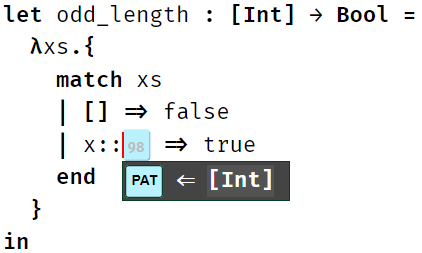
\includegraphics[scale=0.5]{imgs/maybe_exhaustive.png}
		\hfil
		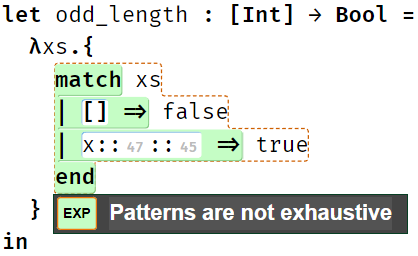
\includegraphics[scale=0.5]{imgs/not_exhaustive.png}
	\end{figure}
\end{frame}

\begin{frame}
\frametitle{Constraint Language}
% !TeX root = presentation.tex

\begin{figure}[ht]
$\arraycolsep=4pt\begin{array}{lll}
\xi & ::= &
  \ctruth ~\vert~
  \cfalsity ~\vert~
  \cunknown ~\vert~
  \cnum{n} ~\vert~
  \cnotnum{n} ~\vert~
  \cand{\xi_1}{\xi_2} ~\vert~
  \cor{\xi_1}{\xi_2} ~\vert~
  \cinl{\xi} ~\vert~
  \cinr{\xi} ~\vert~
  \cpair{\xi_1}{\xi_2}
\end{array}$
\end{figure}

\begin{itemize}
\item Each pattern $p$ emits a constraint $\xi$ describing the restriction $p$ places on expressions that match it.
\medskip
\begin{itemize}
	\item $x$ and $\_$ emit $\ctruth$
	\medskip
	\item $\heholep{w}$ and $\hholep{p}{w}{\tau}$ emit $\cunknown$
	\medskip
	\item If $p_1$ emits $\xi_1$ and $p_2$ emits $\xi_2$, then $\hpair{p_1}{p_2}$ emits $\cpair{\xi_1}{\xi_2}$
\end{itemize}
\medskip
\item A sequence of rules emits the $\lor$ of constraints emitted by each rule.
\medskip
\item The dual $\cdual{\xi}$ represents negation
\medskip
\begin{itemize}
	\item $\cdual{\cnum{n}} = \cnotnum{n}$
	\medskip
	\item $\cdual{\cinl{\xi}} = \cor{\cinr{\ctruth}}{\cinl{\cdual{\xi}}}$
\end{itemize}
\end{itemize}
\end{frame}

\begin{frame}
\frametitle{Constraint Satisfaction}
\begin{itemize}
\item For an expression $e$ and constraint $\xi$,
\begin{itemize}
	\item $\csatisfy{e}{\xi}$ - $e$ satisfies $\xi$
	\item $\cmaysatisfy{e}{\xi}$ - $e$ may satisfy $\xi$ (due to holes in $e$ or $\cunknown$ in $\xi$)
	\item $\csatisfyormay{e}{\xi}$ - $e$ satisfies or may satisfy $\xi$
\end{itemize}
\medskip

\item Possible Exhaustiveness - Every expression possibly matches at least one pattern in the sequence
\begin{itemize}
\item If the rules emit $\xi_{rs}$, then all expressions $e$ have $\csatisfyormay{e}{\xi_{rs}}$.
\end{itemize}
\medskip

\item Necessary Redundancy - Every expression possibly matching $p$ also must match a previous pattern $p^\prime$
\begin{itemize}
	\item If the previous rules emit $\xi_{pre}$ and the current rule emits $\xi_r$, then every expression $e$ with $\csatisfyormay{e}{\xi_r}$ also has $\csatisfy{e}{\xi_{pre}}$.
\end{itemize}
\end{itemize}
\end{frame}

\begin{frame}
\frametitle{Constraint Entailment}
\begin{itemize}
\item Redundancy and exhaustiveness can be stated as a form of entailment between constraints
\medskip
\item Indeterminate Entailment - $\csatisfy{\xi_1}{\xi_2}$ if $\csatisfyormay{e}{\xi_1}$ implies $\csatisfy{e}{\xi_2}$.
\smallskip
\begin{itemize}
	\item $\xi_r$ is necessarily redundant with respect to $\xi_{pre}$ if $\csatisfy{\xi_r}{\xi_{pre}}$
\end{itemize}
\medskip
\item Possible Entailment - $\csatisfyormay{\xi_1}{\xi_2}$ if $\csatisfyormay{e}{\xi_1}$ implies $\csatisfyormay{e}{\xi_2}$
\smallskip
\begin{itemize}
\item $\xi$ is possibly exhaustive if $\csatisfyormay{\ctruth}{\xi}$
\end{itemize}
\medskip
\item Problem: How do we actually decide this?
\end{itemize}
\end{frame}

\begin{frame}
\frametitle{Eliminating Indeterminacy}
\begin{itemize}
\item Consider the "most general" hole-fillings to eliminate indeterminacy
\begin{itemize}
	\item $\ctruify{\xi_1} = \xi_2$ - replace every instance of $\cunknown$ with $\ctruth$
	\item $\cfalsify{\xi_1} = \xi_2$ - replace every instance of $\cunknown$ with $\cfalsity$
\end{itemize}

\medskip
\item $\xi$ is possibly exhaustive if and only if $\ctruify{\xi}$ is exhaustive
\medskip
\item $\xi_r$ is necessarily redundant with respect to $\xi_{pre}$ if and only if $\ctruify{\xi_r}$ is redundant with respect to $\cfalsify{\xi_{pre}}$

\begin{figure}
	\centering
	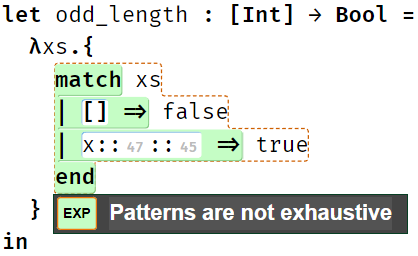
\includegraphics[scale=0.5]{imgs/not_exhaustive.png}
	\hfil
	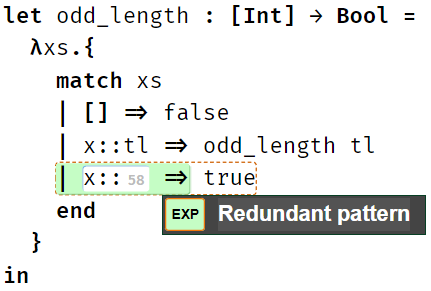
\includegraphics[scale=0.5]{imgs/redundant.png}
\end{figure}
\end{itemize}
\end{frame}

\begin{frame}
\frametitle{Constraint Validity}
\begin{itemize}
\item Inspiration: In classical logic, $P \implies Q$ if and only if $\neg P \lor Q$
\medskip
\item Constraint Validity - Suppose $\xi$ contains no instances of the $?$ constraint. Then $\csatisfy{\;}{\xi}$ if for every $\isVal{e}$ we have $\csatisfy{e}{\xi}$
\medskip
\item Material Implication - If $\xi_1$ and $\xi_2$ contain no instances of $?$, then $\csatisfy{\xi_1}{\xi_2}$ if and only if $\csatisfy{\;}{\cor{\cdual{\xi_1}}{\xi_2}}$
\medskip
\item Redundancy - $\csatisfy{\xi_1}{\xi_2}$ if and only if $\csatisfy{\;}{\cor{\cdual{\ctruify{\xi_1}}}{\cfalsify{\xi_2}}}$
\medskip
\item Exhaustiveness - $\csatisfyormay{\top}{\xi}$ if and only if $\csatisfy{\;}{\ctruify{\xi}}$.
\end{itemize}
\end{frame}

\begin{frame}
	\frametitle{Decision Procedure}
\begin{itemize}
\item For every expression $e$, either $\csatisfy{e}{\xi}$ or $\csatisfy{e}{\cdual{\xi}}$, but not both
\medskip
\item $\csatisfy{\;}{\xi}$ if and only if nothing satisfies $\cdual{\xi}$, i.e. if $\cdual{\xi}$ is inconsistent
\medskip
\item $\csatisfyormay{\ctruth}{\xi_{rs}} \iff \csatisfy{\;}{\ctruify{\xi_{rs}}} \iff \cincon{\cdual{\ctruify{\xi_{rs}}}}$
\medskip
\item $\csatisfy{\xi_r}{\xi_{pre}} \iff \csatisfy{\;}{\cor{\cdual{\ctruify{\xi_1}}}{\cfalsify{\xi_2}}} \iff \cincon{\cdual{\cor{\cdual{\ctruify{\xi_1}}}{\cfalsify{\xi_2}}}}$
\bigskip
\item Reason about inconsistent sets to handle boolean combinations
\medskip 
\begin{itemize}
\item For $\xi_1 \land \xi_2 \land \xi_3$, consider $\{\xi_1, \xi_2, \xi_3 \}$
\medskip
\item For $\xi_1 \land (\xi_2 \lor \xi_3)$, consider $\{\xi_1, \xi_2\}$ and $\{\xi_1, \xi_3\}$.
\end{itemize}

\end{itemize}
\end{frame}

\begin{frame}
	\frametitle{Decision Procedure}
	% !TEX root = thesis.tex

\begin{figure}[ht]
\judgbox{\cincon{\Xi}}{}
\scalebox{0.9}{
\begin{mathpar}
\Infer{\CINCTruth}{
  \cincon{\Xi}
}{
  \cincon{\Xi, \ctruth}
}

\Infer{\CINCFalsity}{ }{
  \cincon{\Xi, \cfalsity}
}

\Infer{\CINCNum}{
  n_1 \neq n_2
}{
  \cincon{\Xi, \cnum{n_1}, \cnum{n_2}}
}

\Infer{\CINCNotNum}{ }{
  \cincon{\Xi, \cnum{n}, \cnotnum{n}}
}

\Infer{\CINCAnd}{
  \cincon{\Xi, \xi_1, \xi_2}
}{
  \cincon{\Xi, \cand{\xi_1}{\xi_2}}
}

\Infer{\CINCOr}{
  \cincon{\Xi, \xi_1} \\
  \cincon{\Xi, \xi_2}
}{
  \cincon{\Xi, \cor{\xi_1}{\xi_2}}
}

\Infer{\CINCInl}{
	\cincon{\setof{\xi' | \cinl{\xi'} \in \Xi},\xi}
}{
	\cincon{\Xi, \cinl{\xi}}
}

\Infer{\CINCInr}{
	\cincon{\setof{\xi' | \cinr{\xi'} \in \Xi},\xi}
}{
	\cincon{\Xi, \cinr{\xi}}
}

\Infer{\CINCInj}{ }{
  \cincon{\Xi, \cinl{\xi_1}, \cinr{\xi_2}}
}

%\Infer{\CINCPairL}{
%    \cincon{\setof{\xi_1' | \cpair{\xi_1'}{\xi_2'} \in \Xi},\xi_1}
%}{
%    \cincon{\Xi, \cpair{\xi_1}{\xi_2}}
%}
%
%\Infer{\CINCPairR}{
%    \cincon{\setof{\xi_2' | \cpair{\xi_1'}{\xi_2'} \in \Xi},\xi_2}
%}{
%    \cincon{\Xi, \cpair{\xi_1}{\xi_2}}
%}
\end{mathpar}
}
\end{figure}

\end{frame}

\begin{frame}
\frametitle{Mechanization}
\begin{itemize}
\item Proofs are often difficult to verify, tedious, and casework-heavy
\medskip
\begin{itemize}
	\item Yongwei intially typed out $\sim 150$ pages of proofs!
\end{itemize}
\medskip
\item Agda proof-assistant allows us to mechanize our proofs, and type-checking shows correctness
\medskip
\item Use fancy dependent type system in order to
\medskip
\begin{itemize}
	\item encode each judgement as a type whose terms are derivations
	\medskip
	\item encode each theorem as a type whose terms are proofs
\end{itemize}
\medskip
\item A function $f : P \to Q$ proves an implication - it gives you a proof of $Q$ whenever you give it a proof of $P$
\end{itemize}
\end{frame}

\begin{frame}{Mechanization}
\begin{lemma}[Matching Determinism]
	\label{lemma:match-determinism}
	If $\isFinal{e}$ and $\hexptyp{\cdot}{\Delta}{e}{\tau}$ and $\hpattyp{p}{\tau}{\Gamma}{\Delta}$ then exactly one of the following holds
	\begin{enumerate}
		\item $\hpatmatch{e}{p}{\theta}$ for some $\theta$
		\item $\hmaymatch{e}{p}$
		\item $\hnotmatch{e}{p}$
	\end{enumerate}
\end{lemma}

\begin{lemma}[Matching Coherence of Constraint]
	\label{lemma:const-matching-coherence}
	Suppose that $\hexptyp{\cdot}{\Delta_e}{e}{\tau}$ and $\isFinal{e}$ and $\chpattyp{p}{\tau}{\xi}{\Gamma}{\Delta}$. Then we have
	\begin{enumerate}
		\item $\csatisfy{e}{\xi}$ iff $\hpatmatch{e}{p}{\theta}$
		\item $\cmaysatisfy{e}{\xi}$ iff $\hmaymatch{e}{p}$
		\item $\cnotsatisfyormay{e}{\xi}$ iff $\hnotmatch{e}{p}$
	\end{enumerate}
\end{lemma}
\end{frame}

\begin{frame}
\frametitle{Mechanization}
\begin{theorem}[Exclusiveness of Constraint Satisfaction]
	\label{theorem:exclusive-constraint-satisfaction}
	If $\ctyp{\xi}{\tau}$ and $\hexptyp{\cdot}{\Delta}{e}{\tau}$ and $\isFinal{e}$ then exactly one of the following holds
	\begin{enumerate}
		\item $\csatisfy{e}{\xi}$
		\item $\cmaysatisfy{e}{\xi}$
		\item $\cnotsatisfyormay{e}{\xi}$
	\end{enumerate}
\end{theorem}

\begin{theorem}[Exclusiveness of Satisfaction Judgment]
	\label{theorem:exclusive-complete-constraint-satisfaction}
	If $\ctyp{\xi}{\tau}$ and $\hexptyp{\cdot}{\Delta}{e}{\tau}$ and $\isVal{e}$ then exactly one of the following holds
	\begin{enumerate}
		\item $\ccsatisfy{e}{\xi}$
		\item $\ccsatisfy{e}{\cdual{\xi}}$
	\end{enumerate}
\end{theorem}
\end{frame}

\begin{frame}
\frametitle{Mechanization}
\begin{theorem}[Deterministic Progress]
	\label{theorem:determinism}
	If $\hexptyp{\cdot}{\Delta}{e}{\tau}$ then exactly one of the following holds
	\begin{enumerate}
		\item $\isVal{e}$
		\item $\isIndet{e}$
		\item $\htrans{e}{e'}$ for some unique $e'$
	\end{enumerate}
\end{theorem}
\begin{theorem}[Preservation]
	\label{theorem:preservation}
	If $\hexptyp{\cdot}{\Delta}{e}{\tau}$ and $\htrans{e}{e'}$
	then $\hexptyp{\cdot}{\Delta}{e'}{\tau}$
\end{theorem}
\end{frame}

\begin{frame}
\begin{center}
Thank you for listening!
\end{center}
\end{frame}

\end{document}

%%